\begin{enumerate}[label=\thesection.\arabic*,ref=\thesection.\theenumi]

\item Find the points on the curve $x^2+y^2-2x-3=0$ at which the tangents are parallel to the x-axis.
\label{chapters/12/6/3/19}
\\
\solution
	\begin{figure}[H]
		\centering
 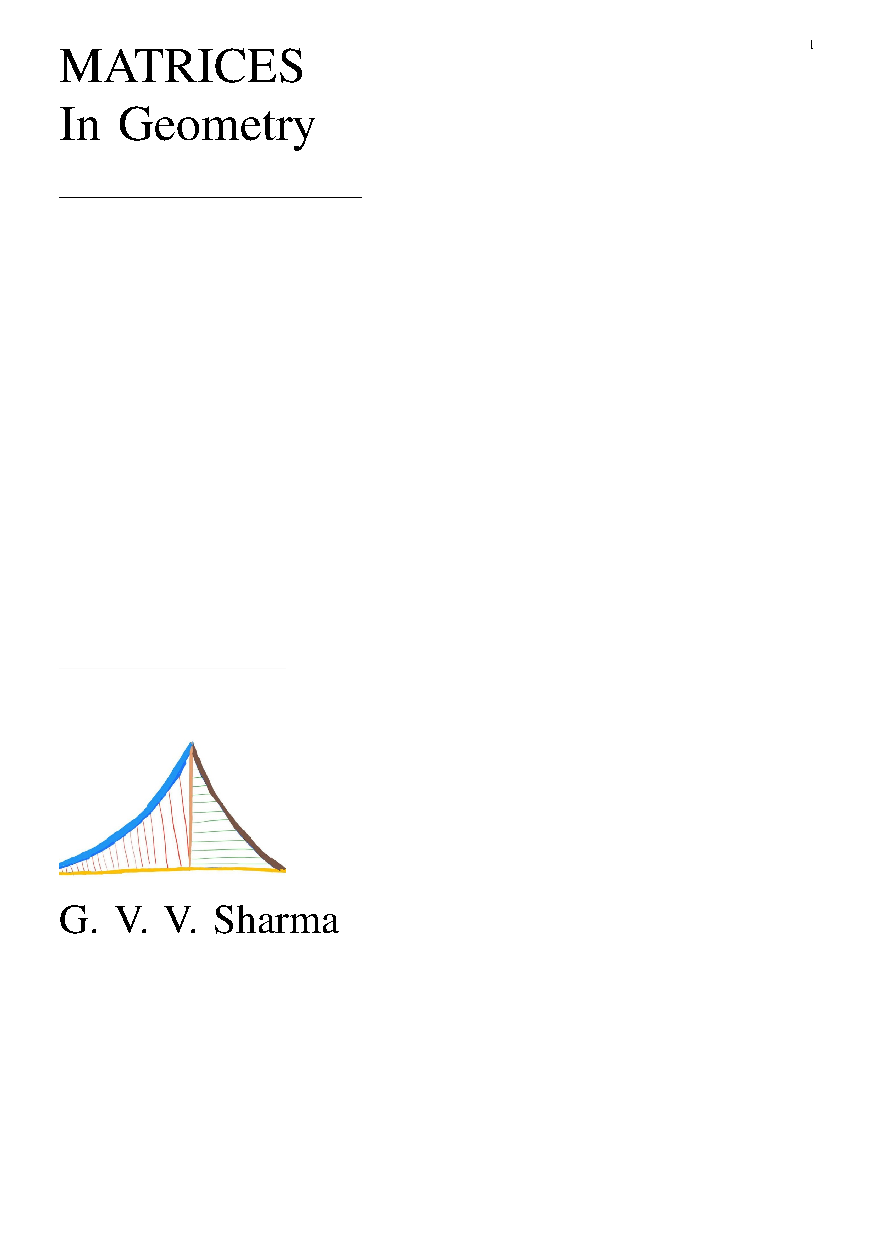
\includegraphics[width=0.75\columnwidth]{chapters/12/6/3/8/figs/main.png}
		\caption{}
		\label{fig:12/6/3/8}
  	\end{figure}
The equation of the conic can be represented as
\begin{align}
\vec{x}^{\top}\myvec{1&0\\0&0}\vec{x}+2\myvec{-2&\frac{-1}{2}}\vec{x}+4=0
\end{align}
So,
\begin{align}
\vec{V}=\myvec{1&0\\0&0},
\vec{u}^{\top}=\myvec{-2&\frac{-1}{2}},
f=4
\end{align}
The direction vector of the line passing through (2,0) and (4,4) is 
\begin{align}
\vec{m}=\myvec{1\\2}
\implies
\vec{n}=\myvec{2\\-1}.
\end{align}
The eigenvector corresponding to the zero eigenvalue is 
\begin{align}
\vec{p}_1=\myvec{0\\1},
\end{align}
In
\eqref{eq:conic_tangent_q_eigen},
\begin{align}
	\kappa=\frac{\myvec{0&1}\myvec{-2\\ \frac{-1}{2}}}{\myvec{0&1}\myvec{2\\-1}}
	=\frac{1}{2}
\end{align}
Substituting  $\kappa$,
from 
\eqref{eq:conic_tangent_q_eigen},
\begin{align}
	\myvec{\sbrak{\myvec{-2\\\frac{-1}{2}}+\frac{1}{2}\myvec{2\\-1}}^{\top} \\ \myvec{1&0\\0&0}}\vec{q} &= \myvec{-4 \\ \frac{1}{2}\myvec{2\\-1}-\myvec{-2\\\frac{-1}{2}}}\\
	\implies
	\myvec{-1&-1 \\ 1&0 \\ 0&0}\vec{q}&=\myvec{-4 \\ 3 \\ 0}
\end{align}
yielding
\begin{align}
\myvec{-1&-1 \\ 1&0}\vec{q} = \myvec{-4\\3}
\end{align}
The augmented matrix is 
\begin{align*}
  \myvec{
                -1&-1&\vrule&-4\\
	        1&0&\vrule&3}
  \xleftrightarrow[]{R_1 \leftarrow R_1+ 2R_2}
     \myvec{
	         1&-1&\vrule&2\\
	         1&0&\vrule&3}
      \\
 \xleftrightarrow[]{R_2 \leftarrow R_2 - R_1}
     \myvec{
	         1&-1&\vrule&2\\
	         0&1&\vrule&1}
 \xleftrightarrow[]{R_1 \leftarrow R_1 + R_2}
     \myvec{
	         1&0&\vrule&3\\
	         0&1&\vrule&1}
      \\ \implies \vec{q}=\myvec{3\\1}
\end{align*}
which is the desired 
point of contact.
See Fig. 
		\ref{fig:12/6/3/8}.

\item Find the equation of a circle of redius 5 which is touching another circle $x^2+y^2-2x-4y-20=0$ at (5,5).
\item The equation of the circle having centre at (3,-4) and touching the line $5x+12y-12=0$ is \makebox[1cm]{\hrulefill}                     
 \item Find the equation of the circle which touches both the axes in first quadrant and whose radius is $a$.
 \item Find the equation of the circle which touches x-axis and whose centre is $(1,2)$
 \item lf the lines $3x-4y+4=0$ and $6x-8y-7=0$ are tangents to a circle, then find the radius of the circle.
 \item Find the equation of a circle which touches  both the axes and the line $3x-4y+8=0$ and lies in the third quadrant.
\item At what points on the curve $x^2+y^2-2x-4y+1=0$, the tangents are parallel to the y-axis?
\item The shortest distance from the point (2,7) to the circle $x^2+y^2- 14x-10y-151=0$ is equal to 5.
\item lf the line $lx+my=1$ is a tangent to the circle $x^2+y^2=a^2$, then the point $(1,m)$ lies an a circle.

\end{enumerate}
